\ffigbox[\FBwidth]{%
\caption{\centering Représentation graphique des contraintes sur \(P\)}\label{Fig:cc_1_ex_1}
}{
    \fbox{
        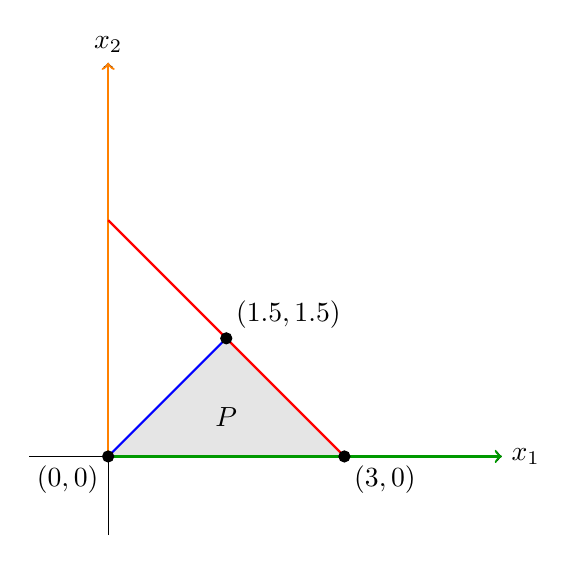
\begin{tikzpicture}[scale=1]
                % Feasible region
                \fill[black!10] (0,0) -- (1.5,1.5) -- (3,0) -- cycle;
                
                % Axes
                \draw[->] (-1,0) -- (5,0) node[right] {\(x_1\)};
                \draw[->, draw=green!60!black, thick] (0,0) -- (5,0) node[right] {};
                \draw[->] (0,-1) -- (0,5) node[above] {\(x_2\)};
                \draw[->, draw=orange, thick] (0,0) -- (0,5) node[above] {};
                
                
                % Constraints
                \draw[thick, draw=red] (0,3) -- (3,0) node[midway, above right] {};
                \draw[thick, draw=blue] (0,0) -- (1.5,1.5) node[midway, above left] {};
                
                
                % Points extrêmes 
                \filldraw[] (0,0) circle (2pt) node[below left] {\((0,0)\)};
                \filldraw[] (1.5,1.5) circle (2pt) node[above right] {\((1.5,1.5)\)};
                \filldraw[] (3,0) circle (2pt) node[below right] {\((3,0)\)};

                % Centre du polytope
                \node at (1.5,0.5) {\(P\)};
            \end{tikzpicture}
    }
}